%%==========================
%% chapter01.tex for TJU Master Thesis
%% based on CASthesis
%% modified by charlie.yaha@gmail.com
%% version: 0.1alpha
%% Encoding: UTF-8
%% last update: Dec 5th, 2010
%%==================================================

%\bibliographystyle{TJU} %[此处用于每章都生产参考文献]


\chapter{绪~论}
\label{chap:introduintroduction}
\section{研究背景}

\cite{Potluri2006}


%了解什么事软管
\section{软管组件简介}
%软管定义,软管组件结构
编织加强软管由内管、纤维增强层及金属连接件组成,是一种复合结构的管路连接件,一般将整个系统结构称为软管组件(Flexible Hose Assembly),或软管总成(本文统一称为软管组件)。
其结构如图\ref{fig:hose structure}所示:柔性内管,例如橡胶管,氟塑料管,热塑料管,金属波纹管,其外外包覆若干层柔性加强结构(编织、缠绕),主要承受内管的内压荷载,加强层数一般视内压荷载大小而定。软管组件工作时,绝大部分内压荷载由编织层承担,内管主要起通道的作用。


\begin{figure}[!htbp]
\centering
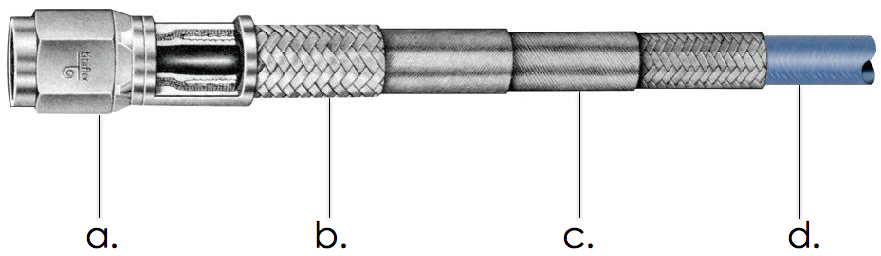
\includegraphics[width=0.6\linewidth]{figure/chap1/Hose-Structure}
\bicaption[fig:hose structure]{软管组件结构}{软管组件结构(a.接头,b.金属纤维编织层,c.金属纤维缠绕层,d.内管)}{Fig}{Hose Structure(a.Coupling,b.Braid Layer,c.Helix-wound Layer,d.Inner Tube)}
\label{fig:hose structure}
\end{figure}


软管组件主要应用于液压、气动、燃油、滑油等系统的介质传输,起到了“血管”作用,航空航天飞行器、汽车、船舶,以及各种工业设备、机床等,都大量使用了软管组件。如图\ref{fig:plane-hose}所示,飞机液压系统(\ref{fig:plane-cruit})



%在刚性管无法使用的情况下使用:
%\begin{itemize}
%	\item 持续的运动
%	\item 振动
%	\item 冲击
%	\item 任意排列
%	\item 高压和压力的释放
%\end{itemize}

软管组件是液压传动系统中非常重要的组成部分。相比普通硬质管,软管组件可以承受相对较大的内压、轴向荷载,同时保持较小的质量、弯曲刚度,带来以下优势:可以减小系统的刚度,吸收液压源产生的振动;安装方式灵活,节约了系统内部的空间。


\begin{figure}[!htbp]
	\centering
%	\subfigure[起落架]{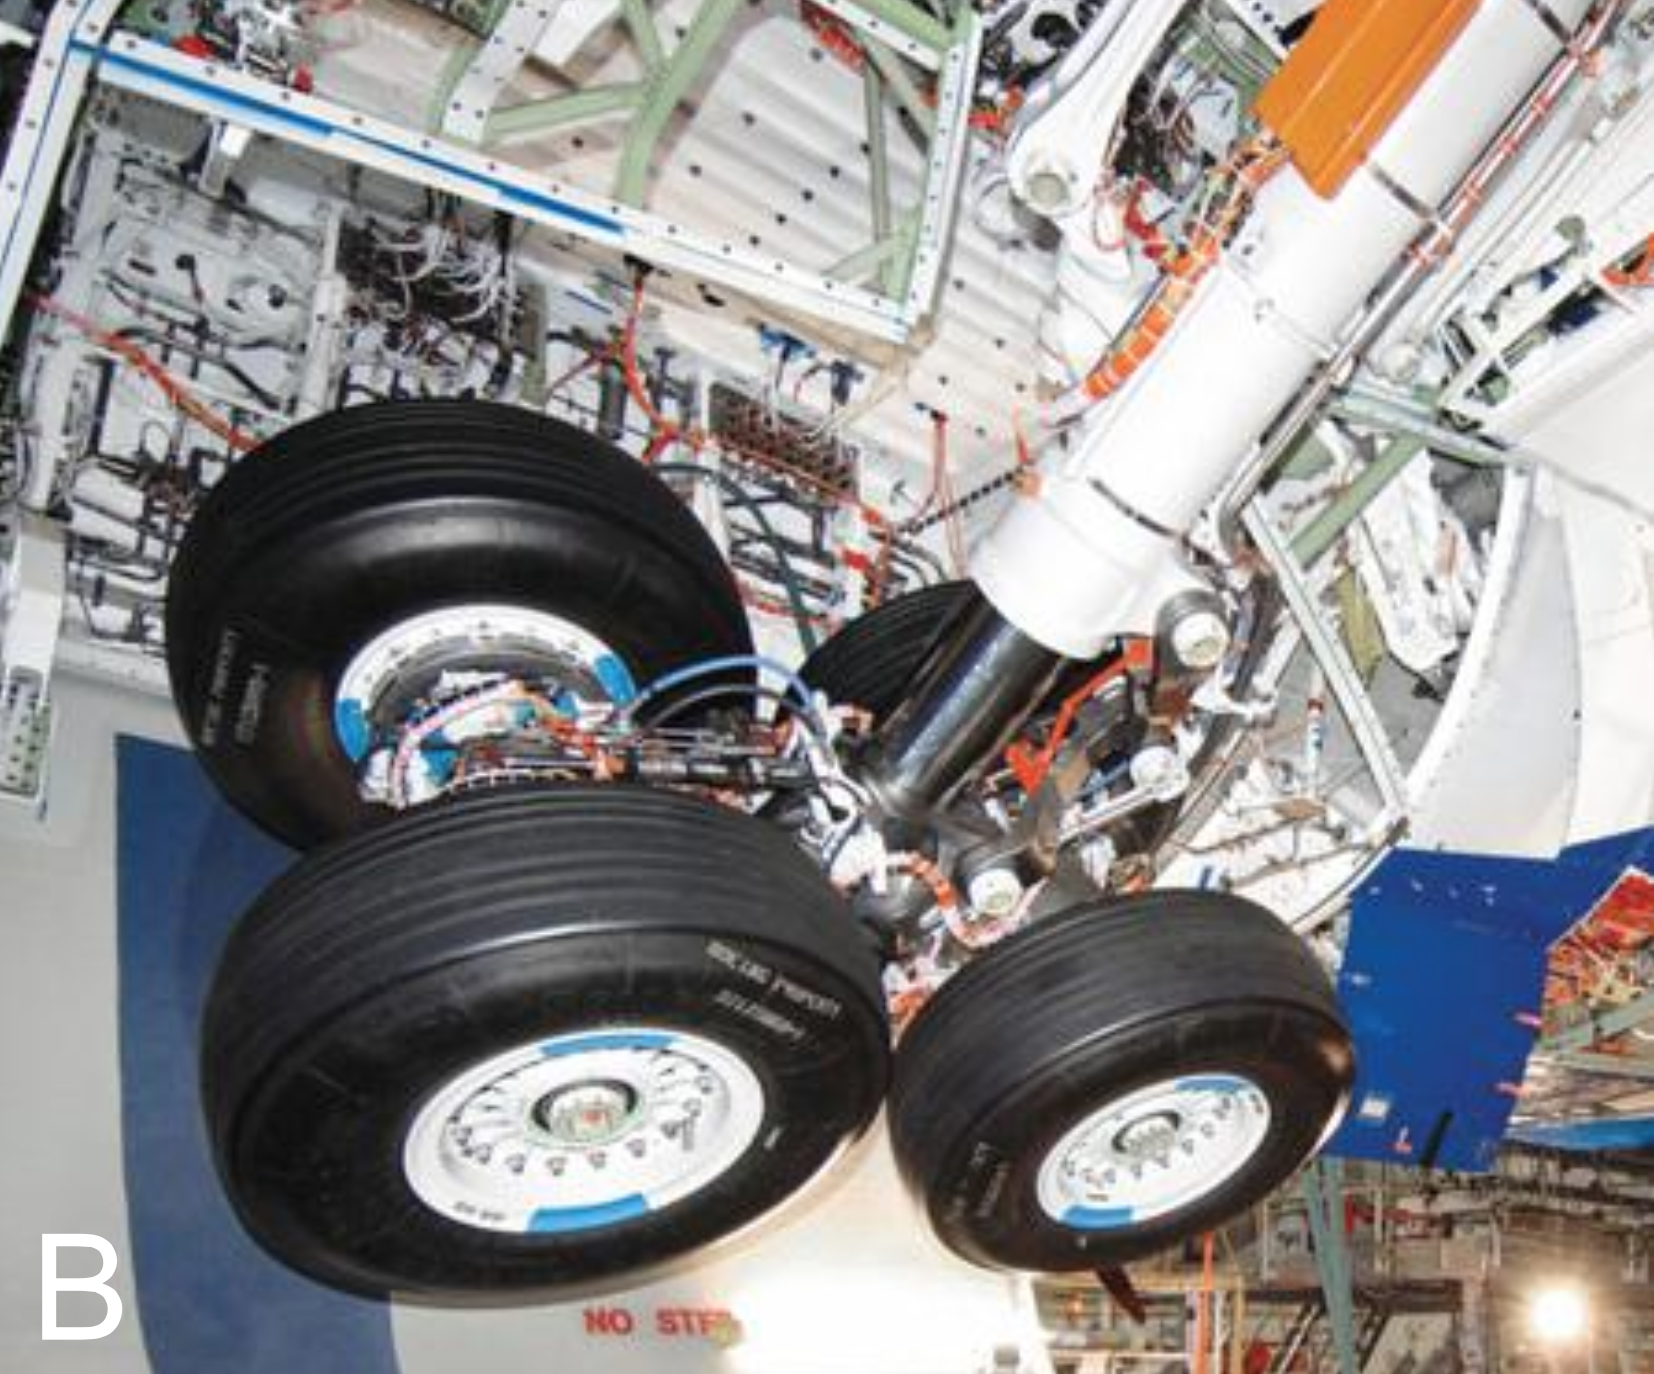
\includegraphics[width=0.4\textwidth]{figure/chap1/gear}}		\label{fig:plane gear}
%	\hspace{1cm}
%	\subfigure[飞机管路]{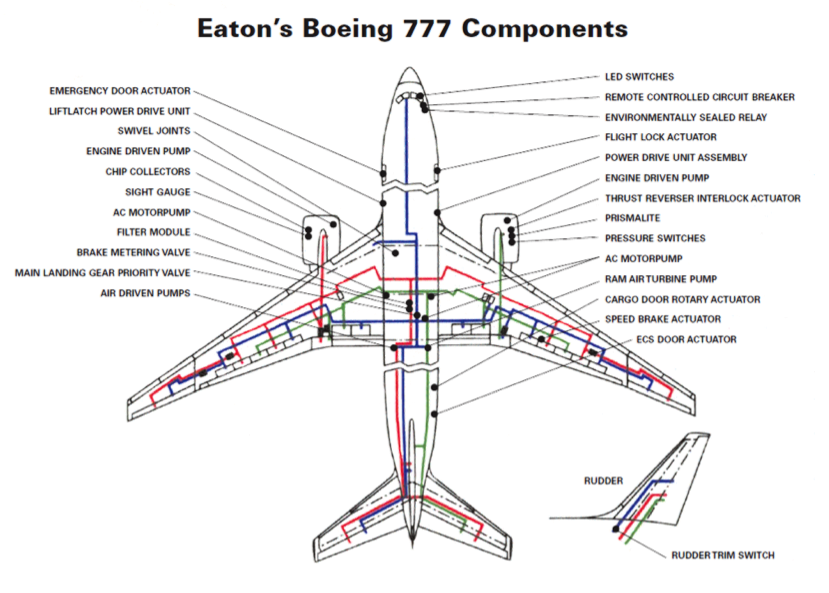
\includegraphics[width=0.5\textwidth]{figure/chap1/Plane}}    \label{fig:plane}
	\subfigure[机身软管管路(a.软管,b.液压源)]{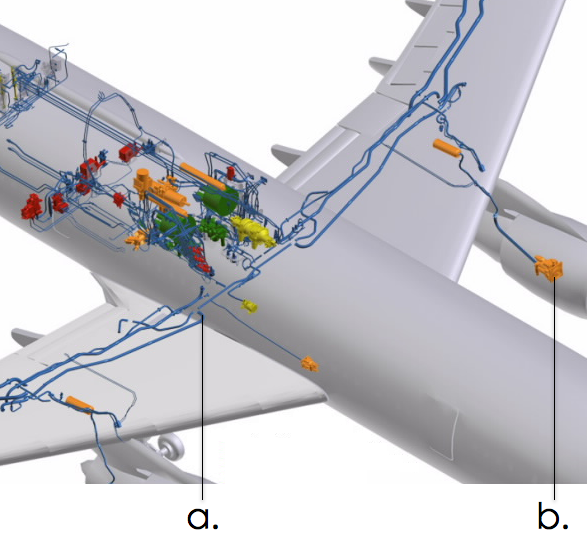
\includegraphics[width=0.4\textwidth]{figure/chap1/plane-cruit}\label{fig:plane-cruit}}    
	\hspace{1cm}
	\subfigure[发动机软管管路(a.软管,b.液压源)]{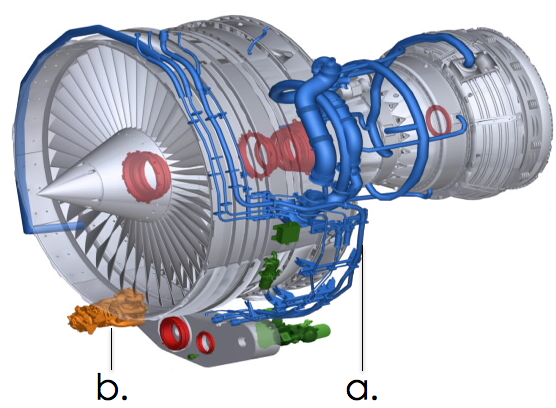
\includegraphics[width=0.4\textwidth]{figure/chap1/engine-cruit}\label{fig:engine-cruit}}    
	\bicaption[fig:SRR]{这里将出现在插图索引中}{飞行器软管组件分布}{Fig}{Distribution of hose assembly in a plane}  
	\label{fig:plane-hose}
\end{figure}


%软管优势



%不同软管型号
软管组件根据不同的口径、编织加强层的层数、重量等参数有以下分类方法:重型、中型、轻型;低压、中压、高压。
重型管管径一般达到20mm,轻型管管径一般在10mm以下;
高压管一般爆破压力要求达到\SI{80}{\mega\pascal},低压管爆破压力一般在40MPa以下。
不同型号的软管对于着不同的工作环境,如以下表\ref{tab:hosefixposition}所示,




\begin{table}[!htbp]
	\centering
	\bicaption[tab:hosefixposition]{testtest}{不同型号软管组件安装位置}{Fig}{Position}
		
	\begin{tabular}{ccc}
		\toprule
		&    轻型     &     重型     \\ \hline
		低压 & 汽车刹车、转向传动 &  输运水、气  \\
		高压 & 飞机起落架、襟翼  & 飞机、船舶液压泵出口 \\ 
		\bottomrule
	\end{tabular} 
\end{table}

%解释表格
飞机、船舶液压泵出口处压强高,流量大,震动强,工作环境极为恶劣,因此国内外一般都采用重型高压软管组件,技术也都已经较为成熟。
飞机起落架、襟翼等部位处于机身液压系统的末端,但压强仍然很高,而且软管的安装空间很小,要求软管组件具有较小的弯曲半径。保持较高的爆破压力的同时,使得软管组件小型化、轻型化,这就对软管组件的设计水平提出了很高的要求。国外企业在轻型高压软管组件领域技术优势明显,基本垄断了该市场。

汽车领域也大量使用了软管组件,例如刹车制动管,转向传动管,空调管等。相比飞行器的液压系统,汽车的液压系统压强较低,如刹车制动管的爆破压力一般为35MPa至40MPa\footnote{GB 16897-2010}。但汽车行业对成本较为敏感,要求在保证设计指标的同时,使软管的结构达到最优化。这对软管的设计、制造也提出了很高的要求。

%软管材质
根据软管寿命、工作环境温度











编织加强层由编织机缠绕于内管之上:若干根金属纤维穿过编织机锭子合为一股,由锭子携带,在圆周上的相互穿插交叠形成编织层。
金属编织软管一般采用2×2的编织(twill)形式(如图 1(c)),这是因为金属纤维一般刚度较大,这种编织形式中每股纤维的曲率较小,可以减小金属纤维所受的应力。

 	 	 
					
\section{研究现状}

纤维编织加强软管的加工生产技术经过几次重大变革,至今为止,已经发展出了3代产品
%第一代
编织加强胶管

%第二代
金属增强软管组件是由美国发明并于上世纪60年代开始用于飞机的液压系统,到上世纪90年代中期,已经广泛应用于航空、航天领域。为此,美国建立了一系列的军用、宇航产品技术标准或规范,例如:MIL-H-25579E、SAE AS604、SAE AS614等。其产品的最高使用温度为232℃,最高工作压力已经达到56MPa。目前广泛应用于各种类型的飞机和导弹、运载火箭等,例如:F-16、F-22、波音客机等。
%第三代
近年来,随着航空航天事业的飞速发展,对为之配套的聚四氟乙烯软管组件也提出轻量化的要求,传统钢丝增强软管组件已不能满足航空航天的设计要求。为了解决这个问题,非金属增强软管组件得到了大力发展,以美国为例,Titeflex、Eaton及Parker等国际知名公司纷纷研制出了各自的非金属增强软管组件产品,并广泛应用在波音、空客和达索等公司的军用、民用飞机上。Parker公司在本世纪初推出了Stratoflex 3154、Stratoflex 3190、Stratoflex 3191和Stratoflex 3192四种型号的非金属编织增强软管组件(见图2),产品的编织增强层根据不同的耐压等级采用不同材料,最高性能产品为耐压等级满足SAE AS1975规范要求的Stratoflex 3154产品采用Kevlar编织,最高工作压力为4000psi(28MPa)。Titeflex及Eaton也紧随其后,推出了自己的非金属编织增强软管组件产品。Titeflex公司主要有TITEFLEX 500、TITEFLEX RA170和TITEFLEX R270三种产品(见图3),最高可满足SAE AS5951规范要求的5080psi(35MPa),产品同样也采用Kevlar编织;Eaton的非金属编织增强软管组件产品型号为AE319、AE334和AE355(见图4),可满足SAE AS5951规定的5080psi(35MPa)工作压力要求。



目前对金属编织加强软管的研究,多见于汽车工业中的中刹车管[2]、转向传动管[3]、空调管[4]等。对软管加强层理论的研究,基本使用通过加强层的总体的要是通过软管理论主要有两个分支[5]:一种是加强层含量较低,橡胶管起主要作用的软管,由Kuipers等人[6,7]提出并完善,适用于帘线加强的软管;另一种是编织加强层主要承力的软管,主要研究的是钢丝螺旋缠绕加强层。软管轴向受拉时,缠绕的金属丝会沿缠绕方向“流动”。编织加强层仅作为螺旋缠绕的一种特例:两层缠绕方向相反,且不允许“流动”的缠绕层[5]。
近20年对编织加强结构的研究主要集中在复合材料编织。复合材料纤维编织的与金属纤维编织的传力机制差别非常明[8]:复合材料纤维只承受单向应力;而金属编织层中的金属丝间的接触关系会直接影响编织层整体的传力,不能忽视。因此,并没有至今尚没有成熟、独立,考虑金属丝间接触关系的编织加强层理论。
有学者尝试用连续介质力学的基本理论推导编织层的本构,如Evans[5]编织层金属纤维侧向传力机制,Horgan等人[9]提出了纤维加强材料的应变能密度函数,国内学者计算了编织结构强度与突加荷载的情况[10,11]。但主流的研究办法还是结合实验,提出能够反映加强层力学行为的有限元模型。Wijaya[4]对包含软管各层材料及编织层的试件进行了压缩实验,认为金属编织层的应力应变关系是线性的,在软管整体动态特性的研究中取得了较好的效果。Cho[3]研究了编织层在扣压安装接头中的力学行为,结合压缩实验提出了弹塑性的本构模型,Rattensperger[8]同样针对压缩的过程,编织层厚度方向引入一组等效非线性弹簧,表征金属纤维间相互作用。
Hachemi[12]对编织层进行了拉伸试验,将复合材料编织中考虑材料非线性行为的特征单元法(首先由Reese[13]提出)引入金属编织层的研究,提出了能够反映编织结构编织角变化的本构模型。该模型将编织层简化两层Rebar单元,只在编织方向上有刚度。但该模型仍然没有考虑两层Rebar单元之间相互接触的关系。

\section{研究内容}
本研究实验表明,Hachemi[12]本构模型的非线性行为并不足够强,不能与本研究中的高压金属编织加强软管的拉伸实验结果相吻合。我们试图通过引入金属纤维间的接触关系来修正该理论与实验的差距。使得包括非线性段的实验结果都能够与修正后的理论值相吻合。
 
